\section{How are decisions made by AIs perceived?}

	\begin{frame}[t]{Perception of AI: Skepticism}
		\textbf{In some studies, people show low acceptance for AI making high stake decisions}
		\begin{itemize}
			\item 58\% of Americans feel that computer programs will always reflect some level of human bias (Smith 2018).
			\item A majority of US Americans consider it unacceptable to use algorithmic decision making in situations with real life consequences (Smith, 2018).
			\item Concerns that they (algorithms) may violate privacy, are unfair, and \textbf{lack nuance} (Smith 2018).
			\item <2> AI is seen as having less agency, and thus are \textbf{less able to make moral decisions}, even when they coincide with humans (Bigman \& Gray, 2018).
			\item <2> Participants found it less permissible for AI to make decisions about life and death driving situations, parole (Bigman \& Gray, 2018).
			\item <2> Participants found it less permissible for AI to make decisions about potentially life-saving, but risky, medical procedures, than a doctor (Bigman \& Gray, 2018).
			\item <2> AI perceived to have less agency and experience, mediating the lower permissibility (Bigman \& Gray, 2018).
		\end{itemize}
		\vspace{-3.5cm}
		\centering
		\begin{tikzpicture}
			\visible<1>{
				\node[inner sep=0pt, draw=black] at (0, 0) {
					\includegraphics[width=4cm]{data/smith.png}
				};

				\node[font=\tiny\selectfont, anchor=south] at (0, -2.77) {
					\href{https://www.pewresearch.org/internet/2018/11/16/public-attitudes-toward-computer-algorithms/}{Public Attitudes Toward Computer Algorithms}, Smith A., \textit{Pew Research Center Newsletter}, 2018
				};
			}
			\visible<2>{
				\node[font=\tiny\selectfont, anchor=south] at (0, -2.77) {
					\href{https://www.researchgate.net/publication/326762041_People_are_Averse_to_Machines_Making_Moral_Decisions}{People are Averse to Machines Making Moral Decisions}, Bigman, Y. E. \& Gray, K., \textit{Cognition}, 2018
				};
			}
		\end{tikzpicture}
	\end{frame}

	\begin{frame}[t]{Perception of AI: Positivism}
		\textbf{In other studies, people show high acceptance for AI making high stake decisions (Araujo et al., 2020)}\\
		A study among a representative sample in the Netherlands asked participants to rate usefulness, fairness, and risk of AI (vs. human) decision-making in the media, health sector, and justice system.
		\begin{itemize}
			\item For high-stake decisions, participants perceived decisions by AI (vs. human) to be more useful, fairer and less risky in health and justice contexts (no difference for low-stake decisions)
			\item Perceived usefulness and fairness increased with knowledge on AI, programming, and algorithms (self-reported).
			\item "... people are by and large concerned about risks and have mixed opinions about fairness and usefulness of automated decision-making at a societal level, with general attitudes influenced by individual characteristics."
		\end{itemize}
		\centering
		\vspace{1.9cm}
		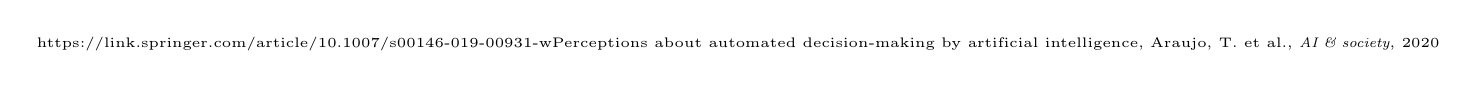
\begin{tikzpicture}
			\node[font=\tiny] at (0, 0) {
				\href{https://link.springer.com/article/10.1007/s00146-019-00931-w}{Perceptions about automated decision-making by artificial intelligence}, Araujo, T. et al., \textit{AI \& society}, 2020
			};
		\end{tikzpicture}
	\end{frame}

	\begin{frame}[t]{Perception of AI: Man vs machine}
		\textbf{More moral outrage when humans discriminate than AI (Bigman et al., 2023)}\\
		Participants were asked to assess degree of discrimination, objectivity, prejudice and moral outrage after reading about a discriminatory hiring process. The discrimination was performed either by an AI or a human (HR specialist).
		\begin{itemize}
			\item When discrimination was performed by the AI, participants perceived the process as more objective, less discriminatory, and less prejudiced.
			\item <2> More moral outrage when the discrimination was performed by a human.
			\item <2> Less permissible that CVs are screened by an algorithm.
			\item <2> Liability of the company was smaller when the biased screening procedure was performed by an AI.
		\end{itemize}
		\only<1>{
			\vspace{-1.6cm}
			\centering
			\begin{tikzpicture}
				\node[inner sep=0pt, draw=black] at (0, 0) {
					\includegraphics[width=5cm]{data/discriminatory_action.png}
				};
				\node[font=\tiny\selectfont] at (0, -3) {
					\href{https://pubmed.ncbi.nlm.nih.gov/35758989/}{Algorithmic discrimination causes less moral outrage than human discrimination}, Bigman, Y. E. et al., \textit{Journal of Experimental Psychology}, 2023
				};
			\end{tikzpicture}
		}
	\end{frame}

	\begin{frame}[t]{Perception of AI: Trust in AI}
		\textbf{What predicts trust in AI (Kaplan et al., 2023)}\\
		A meta-anaylsis was performed across 65 studies that empirically investigated what leads people to trust, defined as "the reliance by an agent that actions prejudicial to their well-being will not be undertaken by influential others" in AI.
		\begin{itemize}
			\item In humans (interacting with the AI), competency, understanding and expertise were the most important factors for facilitating trust.
			\item In the AI itself, reliability was the most important factor, succeeded by performance.
			\item Attributes such as personality, anthropomorphism, behaviour and reputation were also significant predictors of trust.
			\item The context of the relationship between the human and the AI was also important, with the length of the relationship the most important predictor.
		\end{itemize}
		\centering
		\vspace{2.17cm}
		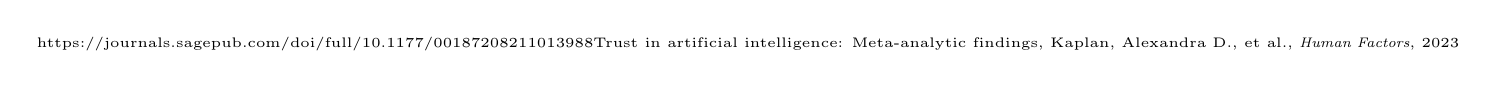
\begin{tikzpicture}
			\node[font=\tiny\selectfont] at (0, -0) {
				\href{https://journals.sagepub.com/doi/full/10.1177/00187208211013988}{Trust in artificial intelligence: Meta-analytic findings}, Kaplan, Alexandra D., et al., \textit{Human Factors}, 2023
			};
		\end{tikzpicture}
	\end{frame}

	\begin{frame}[t]{Perception of AI: Perception of humans?}
		\textbf{Humans overrate their ability to understand eachother (Bonezzi et al., 2022)}\\
		Participants were tasked with evaluating how well they understood the decision process of an agent (human or an AI) performing one of three tasks: (1) evaluating risk for recidivism, (2) examining video interviews, (3) examining a Magnetic Resonance Image to diagnose a disease.
		\begin{itemize}
			\item When only the decision of the agent was made available, without explanation, respondents reported a higher degree of understanding the humans.
			\item This difference was reduced when an explanation was provided alongside the decision.
			\item People project their own decision-making processes onto others.
			\item People overestimate their ability to understand the decision-making processes of other humans.
			\item Could also have a negative effect, e.g. by projecting ones own biases onto others.
			\item <2> \textbf{Are we unfair when asking AIs to explain themselves? Is the only thing that matters predictive proficiency?}
		\end{itemize}
		\only<1>{
			\centering
			\vspace{0.77cm}
			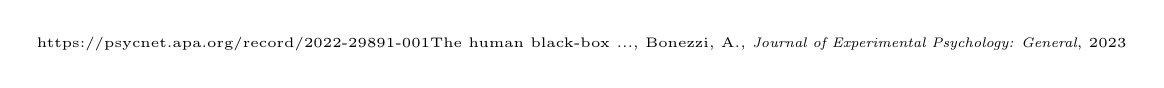
\begin{tikzpicture}
				\node[font=\tiny\selectfont] at (0, -0) {
					\href{https://psycnet.apa.org/record/2022-29891-001}{The human black-box ...}, Bonezzi, A., \textit{Journal of Experimental Psychology: General}, 2023
				};
			\end{tikzpicture}
		}
	\end{frame}

	\begin{frame}[t]{Perception of AI: Summary}
		There is generally a large amount of variability in how people perceive AI (and automated or algorithmic systems in general), and whether they trust their decisions.
		\begin{itemize}
			\item There is a tendency towards not trusting AI to make high-stake decisions, although this varies depending on the exact task at hand, the person doing the trusting, the algorithm being trusted, and the general context.
			\item Although we trust AIs less, we are also less inclined to blame them (or their owners/creators) when they make mistakes, at least morally.
			\item Reliability and performance, both metrics of efficacy, are the most important factors for trust in AI.
			\item Human-like attributes in the AI increase trust.
		\end{itemize}
	\end{frame}

	\begin{frame}{Perception of AI: Ancedote}
		\centering
		\begin{tikzpicture}
			\node[inner sep=0pt, draw=black, label=below:{Generated by DALL-E}] at (0, 0) {
				\includegraphics[width=10cm]{data/robotguide.png}
			};
		\end{tikzpicture}
	\end{frame}

	\begin{frame}{Decision making: Group work}
		What kind of decisions would you be comfortable with AI making on your behalf? What would it take to change your view?
	\end{frame}

	\begin{frame}{Practice questions}
		\begin{itemize}
			\item Explain the differences between narrow and general intelligence.
			\item Explain how AI may lead to biased decisions, although their algorithms are objective mathematical constructs.
			\item Discuss the similarities and dissimilarities between human and artificial intelligence, in terms of their capacities and limitations.
			\item Describe why it is hard to interpret the decisions of modern AI, and what is being done to counteract this.
			\item How do people perceive decisions made by AI systems? Refer to two examples.
		\end{itemize}
	\end{frame}
